\documentclass{beamer}
\usepackage{animate}
\usepackage{graphicx}
\usepackage{pgffor}
\usepackage[T1]{fontenc}
\usepackage{amsmath}
\usepackage[utf8]{inputenc}
\usepackage[german]{babel}
\usepackage[scaled]{helvet}
\usepackage{minted}
%\renew{\familydefault}{\sfdefault}
\usepackage{markdown}
\usepackage{blindtext}
\usepackage{adjustbox}
\usepackage{calc}
\usepackage{listings}
\usepackage{xcolor}
\usepackage{geometry}
\usepackage{longtable}
\usepackage{array}
\usepackage{tabularx}
\usepackage{hyperref,graphicx}
\usepackage{caption}
\usepackage{refstyle}
\usepackage{pdfpages}
\usepackage{comment}
\usepackage{listings}
%\usepackage{xcolor}
%\graphicspath{{bilder/}}
\usepackage{import}
%\usepackage[dvipsnames,table]{xcolor}
%\usepackage{hyperref}
%\us^epackage{multirow}
%\usepackage{textpos}
\usepackage{listings}
\usepackage{color}
\usepackage{tikz}
\usepackage{pgfplots}
\usepackage{ragged2e}
\usepackage{blindtext}
\usepackage{lmodern}
\usepackage[framemethod=tikz]{mdframed}
\usepackage{fixltx2e}
\usepackage{textcomp}
\usepackage{textpos}
\usepackage{tikz}
\usepackage{etoolbox}
\usepackage{listings}
\lstset{
  frame=none,
  xleftmargin=2pt,
  stepnumber=1,
  numbers=left,
  numbersep=5pt,
  numberstyle=\ttfamily\tiny\color[gray]{0.3},
  belowcaptionskip=\bigskipamount,
  captionpos=b,
  escapeinside={*'}{'*},
  language=haskell,
  tabsize=2,
  emphstyle={\bf},
  commentstyle=\it,
  stringstyle=\mdseries\rmfamily,
  showspaces=false,
  keywordstyle=\bfseries\rmfamily,
  columns=flexible,
  basicstyle=\small\sffamily,
  showstringspaces=false,
  morecomment=[l]\%,
}
\lstset{frame=tb,
	language=Java,
	aboveskip=3mm,
	belowskip=3mm,
	showstringspaces=false,
	columns=flexible,
	basicstyle={\small\ttfamily},
	numbers=none,
	numberstyle=\tiny\color{gray},
	keywordstyle=\color{blue},
	commentstyle=\color{darkgreen},
	stringstyle=\color{red},
	breaklines=true,
	breakatwhitespace=true,
	tabsize=3
}


\def\code#1{\texttt{#1}}

\definecolor{darkgreen}{RGB}{0, 100, 0}

\hypersetup{
	colorlinks=magenta,
	linkcolor=blue,
	filecolor=magenta,
	urlcolor=cyan,
	pdftitle={Overleaf Example},
	pdfpagemode=FullScreen,
}

\usetheme{Antibes}
    \setbeamertemplate{footline}[page number]
    \setbeamercovered{transparent=25}
  \setbeamertemplate{navigation symbols}{}
\usecolortheme{dolphin}

\setbeamercolor{item}{fg=cyan}
%\setbeamercolor{section in toc}{fg=cyan}
\setbeamercolor{alerted text}{fg=cyan}
\setbeamercolor{block title}{bg=blue, fg=white}
\setbeamercolor{block body}{bg=lightgray, fg=black}
\definecolor{myblue}{RGB}{0, 102, 104}

\title{Funktionale Programmierung}

%\titlegraphic{
%
\includegraphics[scale=0.1]{nix-snowflake.svg}
%}
\author{Thanh Viet Nguyen}
%\institute[]{Hochschule Hannover}


\begin{document}
\begin{frame}%[plain]
    \maketitle
    \centering
   
\includegraphics[scale=0.15]{bilder/hsh-logo.jpg}[h]
   \date{09.12.2024}

\end{frame}

\begin{frame}
	\tableofcontents
\end{frame}


\section{Einleitung}
\begin{frame}
\begin{itemize}
\item Was ist ein Funktionale Programmierung?
\item Ursprung
\item Unterschiede zur imperativen Programierung
\item Historische Entwicklung
\item Wichtige Konzepte: Funktionen als erste Klasse, Unveränderlichkeit und Rekursion
\item Praktische Beispiele
\item Ziel der Präsentation: grundlägige Verständnis  zur funktionalen Programmierung
\end{itemize}
\end{frame}

\begin{frame}
\frametitle{Weise Worte:}
\begin{itemize}
\item \textmd{"The proper use of comments is to compensate for our failure to express ourselves in code." (Robert C. Martin, Functional Programming in Java, Vorwort)}
\item \textmd{"In programming the hard part isn’t solving problems, but deciding what problems to solve." (Paul Graham, Functional Programming in Java, Vorwort)}
\item \textmd{"Testing by itself does not improve software quality. Test results are an indicator of quality, but
in and of themselves, they don’t improve it. Trying to improve software quality by increasing
the amount of testing is like trying to lose weight by weighing yourself more often." (Steve McConnell, Functional Programming in Java, Vorwort)}
\end{itemize}
\end{frame}


\begin{frame}
	\section{Herkunft der Funktionalen Programmierung}
	\begin{itemize}
		\item Lambda Kalkül (1930):  Alonzo Church (14.06.1903 - 11.08.1995)
		\item Vor Maschinen, die solchen Code ausführen konnten, gab es bereits Ansätze dazu.
        \item Mathematische Themen gebiete: 
        \begin{itemize}
        	\item Typen Theorie
        	\item Kategorie Theorie
        \end{itemize} 
	\end{itemize}
\end{frame}

\begin{frame}{Lambda Kalkül }
		\begin{itemize}
				\item kleinste Universelle Programmiersprache, die keine Machine benötigt
		\end{itemize}
	\begin{align*}
		\langle \text{expression} \rangle & := \langle \text{name} \rangle \mid \langle \text{function} \rangle \mid \langle \text{application} \rangle \\
		\langle \text{function} \rangle & := \lambda \langle \text{name} \rangle . \langle \text{expression} \rangle \\
		\langle \text{application} \rangle & := \langle \text{expression} \rangle \langle \text{expression} \rangle
	\end{align*}
	\end{frame}

\begin{frame}{ Typen Theorie}
 \textmd{Formales System zur Klassifizierung von Objekten in verschiedene Typen, um Paradoxien zu vermeiden, mit einer hierarchischen Struktur, die Typen als Objekte betrachtet, und Anwendungen in der formalen Verifikation, Logik und Grundlagenforschung; oft konstruktivistisch und eng mit intuitionistischer Logik verbunden.}
\begin{itemize}
\item Werte durch Typen klassifiziert, die definieren, welche Art von Daten ein Wert repräsentieren kann.
\item Statische Typisierung: Typen werden zur Compile-Zeit überprüft, was bedeutet, dass viele Fehler frühzeitig erkannt werden können.
\item: Dynamische Typisierung: Typen werden zur Laufzeit überprüft, was mehr Flexibilität bietet, aber auch zu Laufzeitfehlern führen kann. 
\end{itemize}

\end{frame}

\begin{frame}{Kategorie Theorie}
\textmd{Konzept, das Strukturen und Beziehungen zwischen ihnen durch Objekte und Morphismen beschreibt, um verschiedene mathematische Disziplinen zu vereinheitlichen und zu analysieren, wobei zentrale Begriffe wie Funktoren, natürliche Transformationen und Kategorien verwendet werden.}
	\end{frame}

\section{Programmier Paradigmen}
\begin{frame}
	\begin{figure}
	    \centering
	    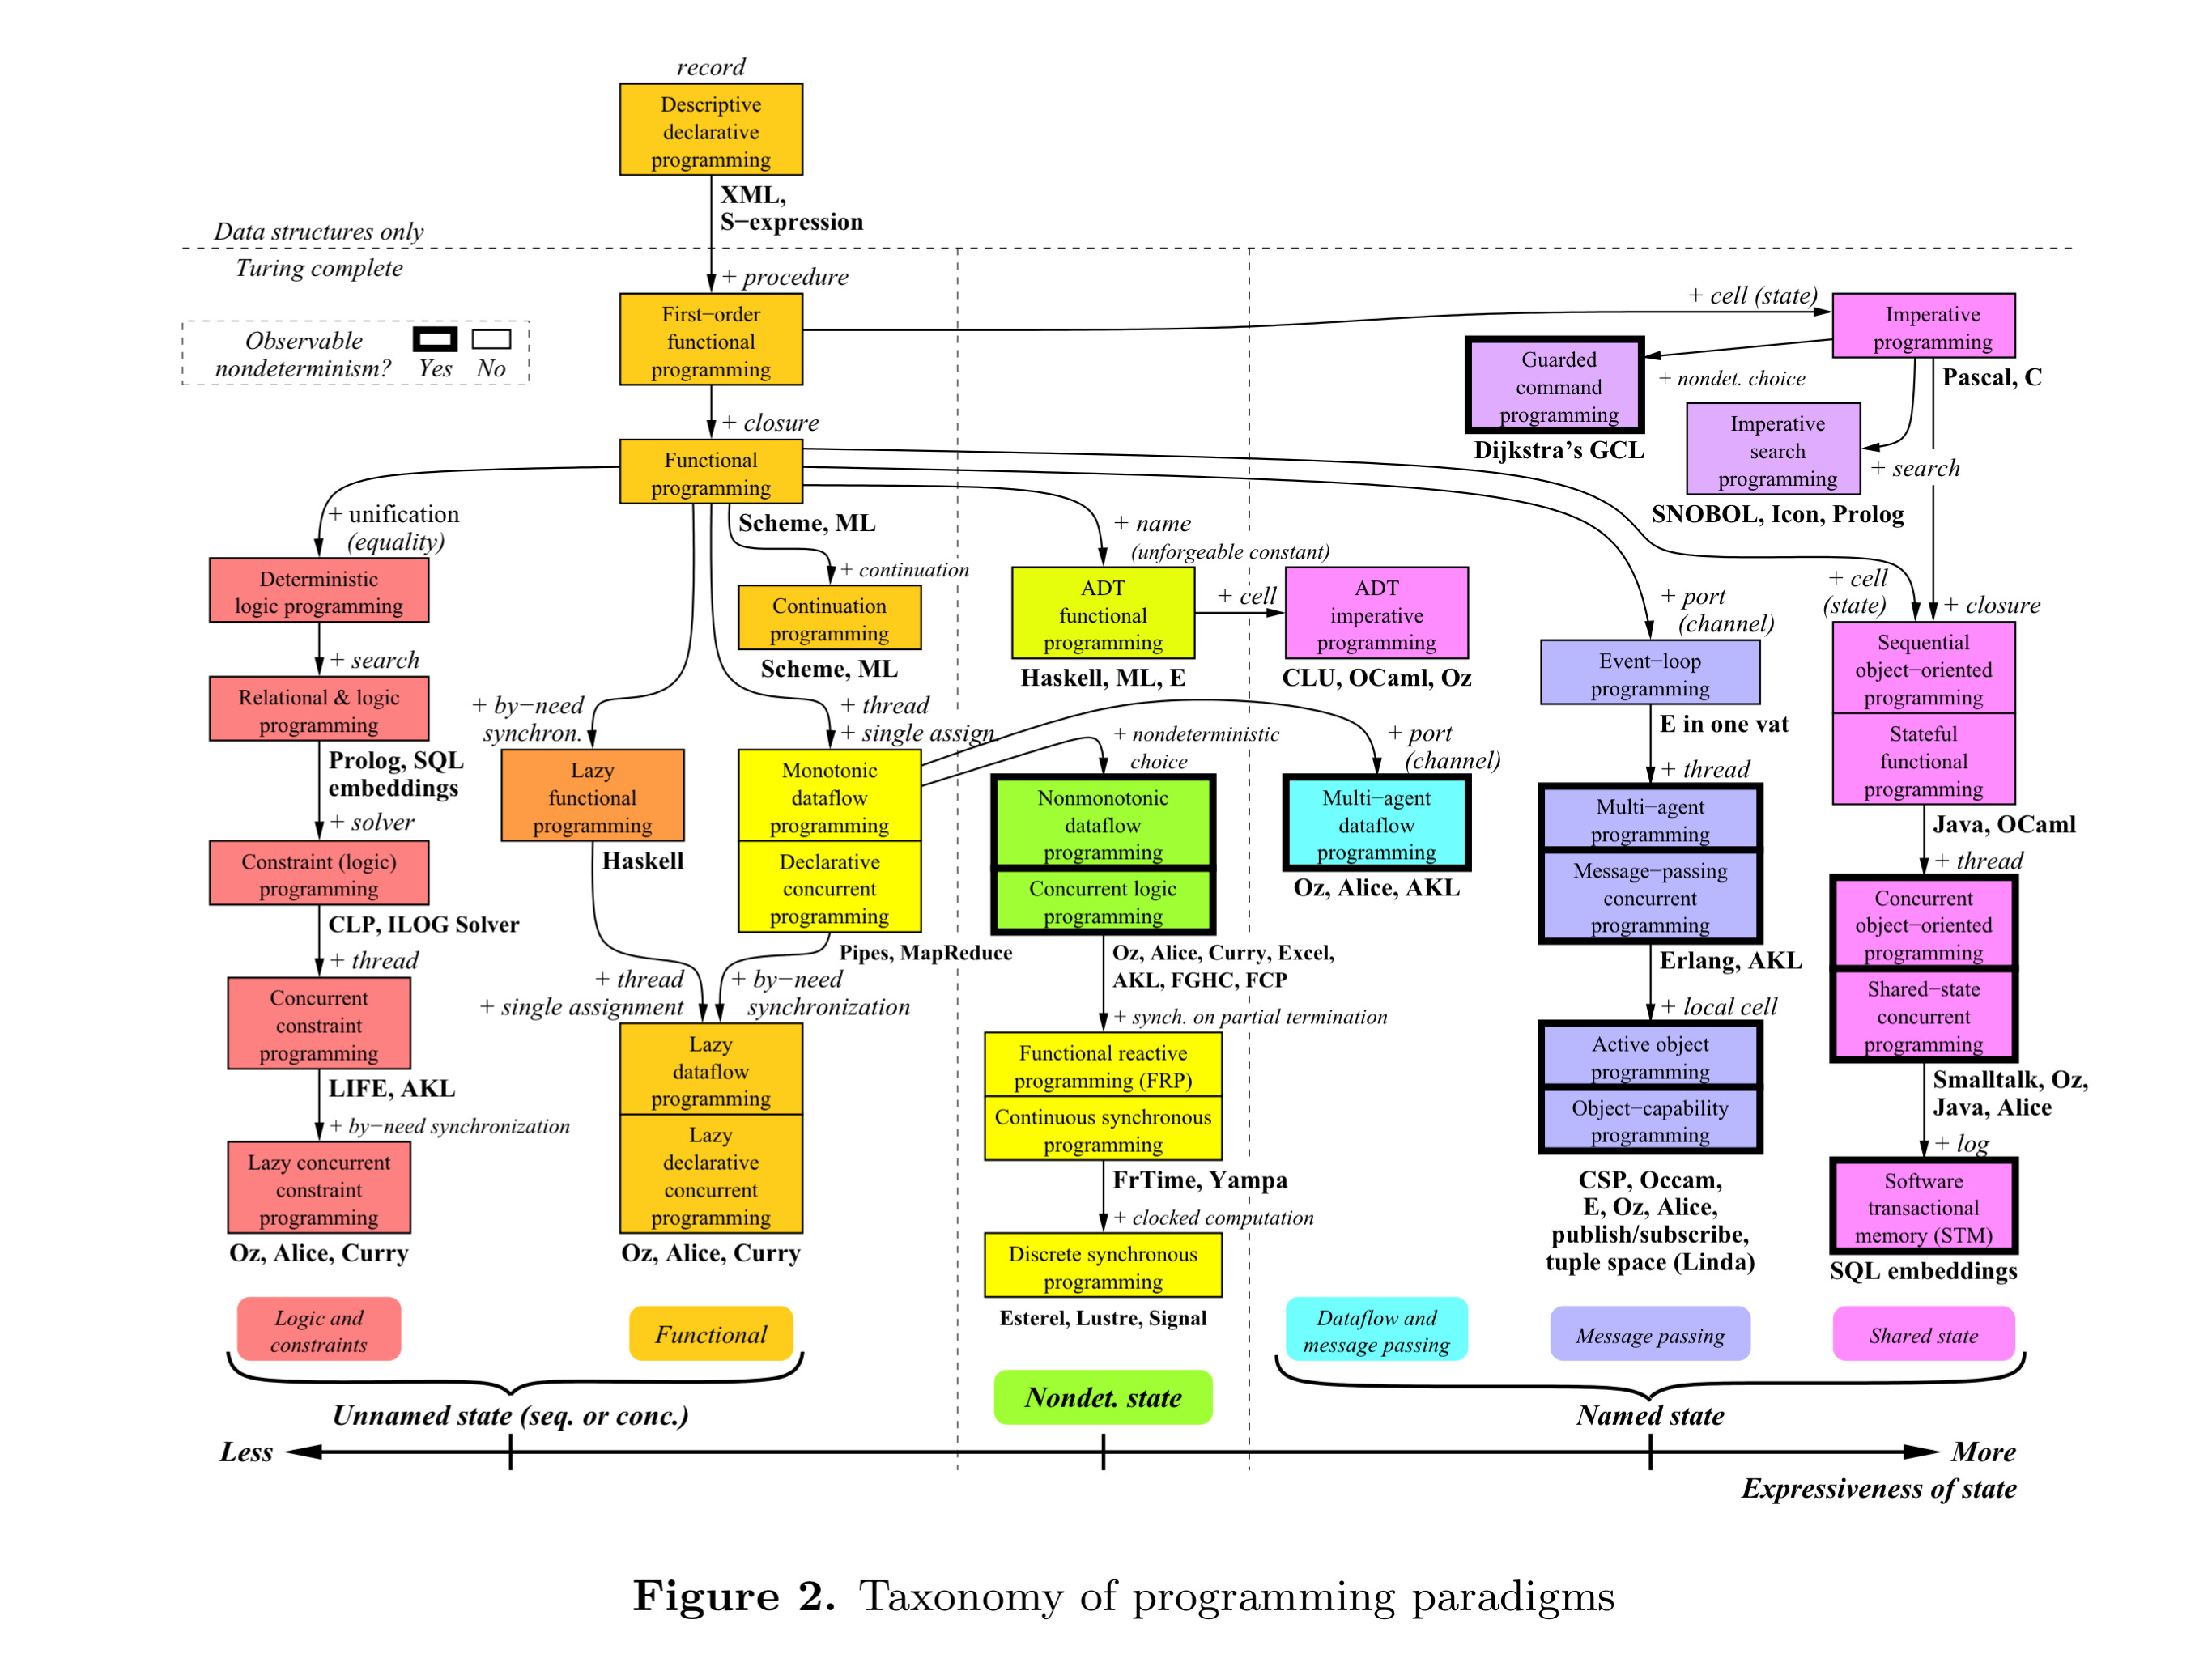
\includegraphics[width=0.9\linewidth]{bilder/Programming-paradigms.png}
	    \textmd{ \tiny https://blog.acolyer.org/2019/01/25/programming-paradigms-for-dummies-what-every-programmer-should-know/}
	    %\label{fig:enter-label}
	\end{figure}
\end{frame}

\begin{frame}{Objekt Orientierung und Funktionale Programmierung}
\begin{figure}
    \centering
    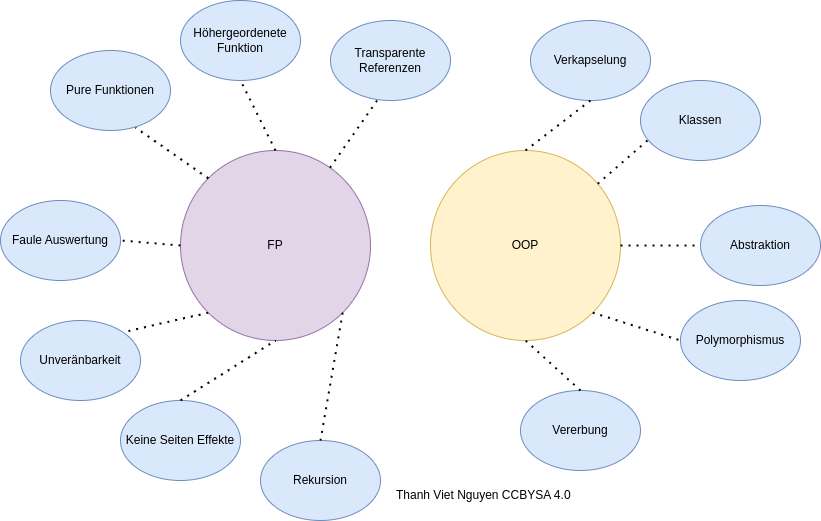
\includegraphics[scale=0.38]{bilder/FPundOOP.drawio.png}
\end{figure}
\end{frame}

\begin{frame}
\begin{figure}
    \begin{itemize}
    \item \textmd{'' Object oriented programming makes code understandable by encapsulating moving parts.
Functional programming makes code understandable by minimizing moving parts.''  \\ 
(Michael Feathers, Functional Programming in Java, Vorwort)}
    \end{itemize}
\end{figure}
\end{frame}

\begin{frame}{Deklaritive und Imperativen Programmiereung}
\centering
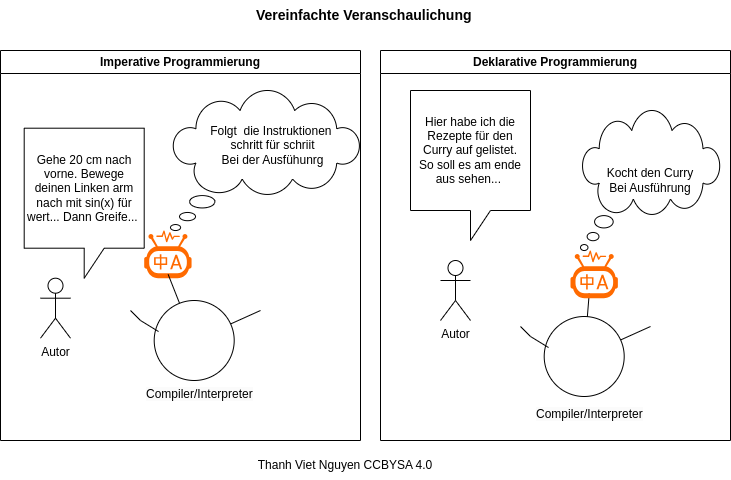
\includegraphics[scale=0.38]{bilder/minicom.drawio.png} 
\end{frame}

\begin{frame}
	\centering
	
\includegraphics[scale=0.35]{bilder/purity.png}
    \textmd{\url{https://xkcd.com/435/}}
\end{frame}

\begin{frame}
	\section{Historie}
\frametitle{Lisp Maschinen}
	\begin{itemize}
            \item 1960er
            \item Hoffnung an Digitales Computing für Mathematischeproblemlösungen 
            \item Erforschung Künstlicher Intelligenz
	\end{itemize}
	    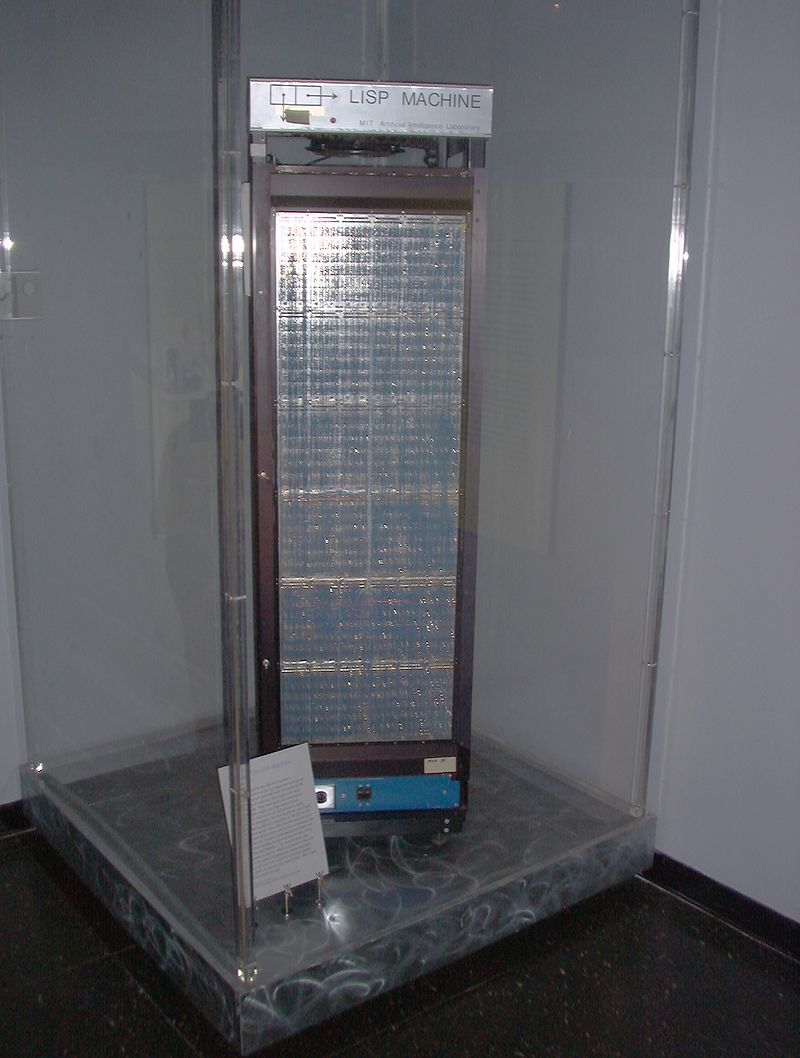
\includegraphics[scale=0.1]{bilder/lispm.jpg}
	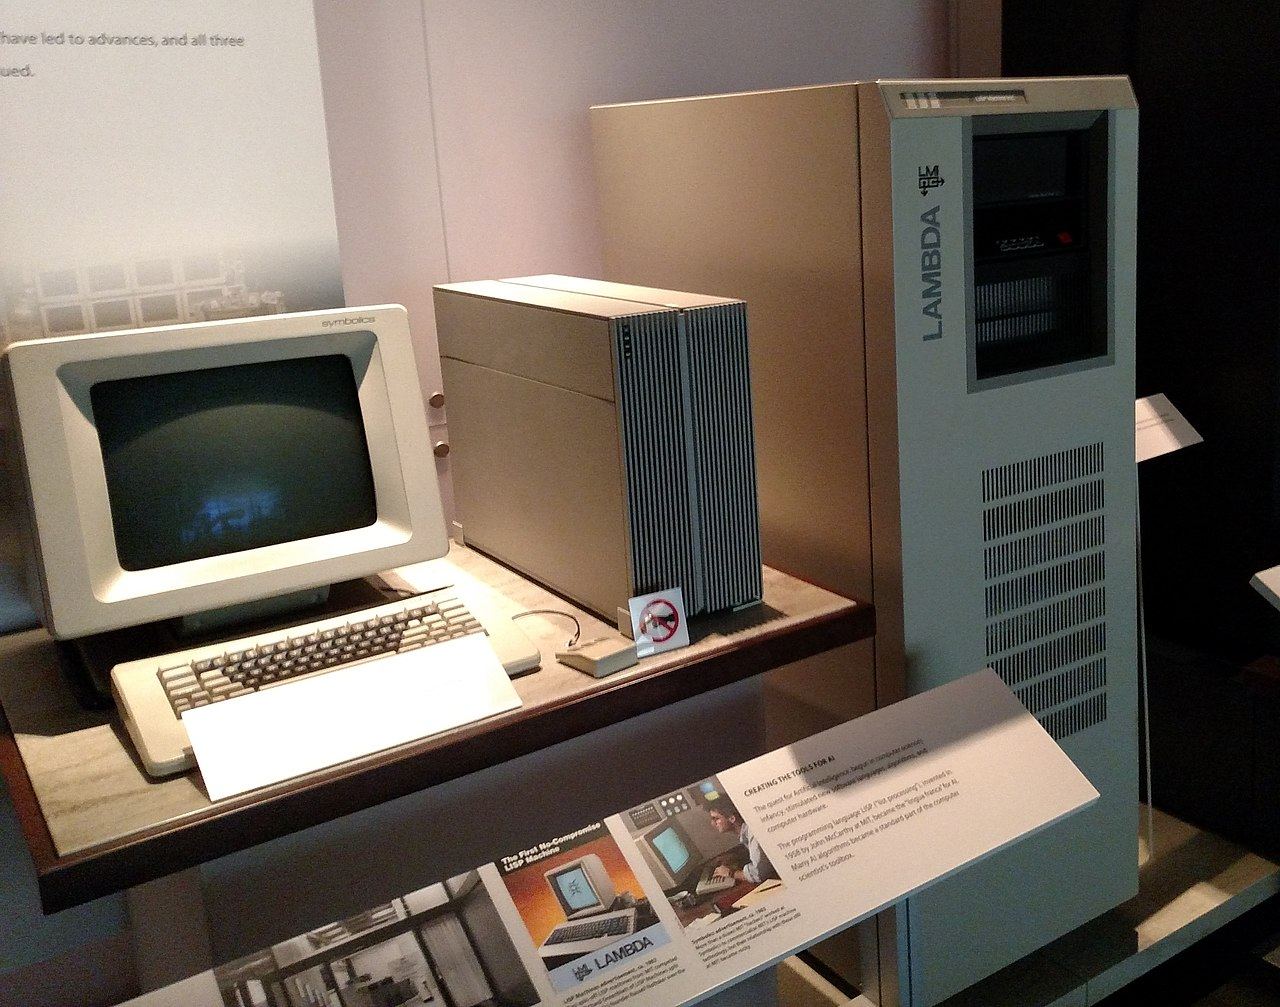
\includegraphics[scale=0.1]{bilder/lispm1.jpg}
	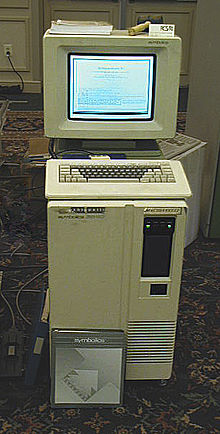
\includegraphics[scale=0.1]{bilder/symblics.jpeg}
	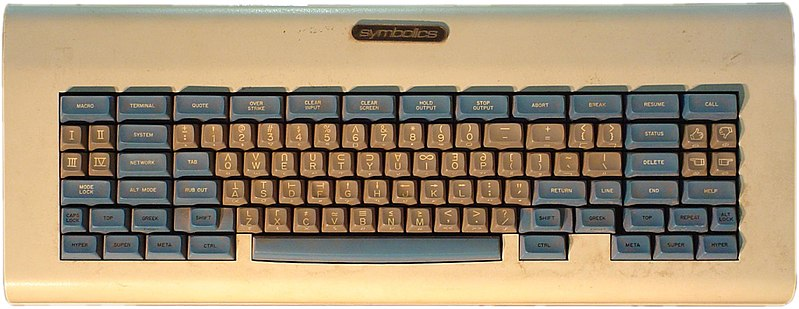
\includegraphics[scale=0.1]{bilder/space.jpg}
	\textmd{\url{https://en.wikipedia.org/wiki/Space-cadet_keyboard} \\ \url{https://en.wikipedia.org/wiki/Lisp_machine} }	
\end{frame}

\begin{frame}
		
\includegraphics[scale=0.1]{bilder/lisp.png}
	   \lstinputlisting[basicstyle=\ttfamily,columns=fullflexible,language=Lisp]{codeBeispiel1/hi.lisp}
	\textmd{\url{https://en.wikipedia.org/wiki/Lisp_(programming_language)}}
\end{frame}

\begin{frame}
\frametitle{Lisp Dialekte}
	\begin{figure}
	    \centering
	    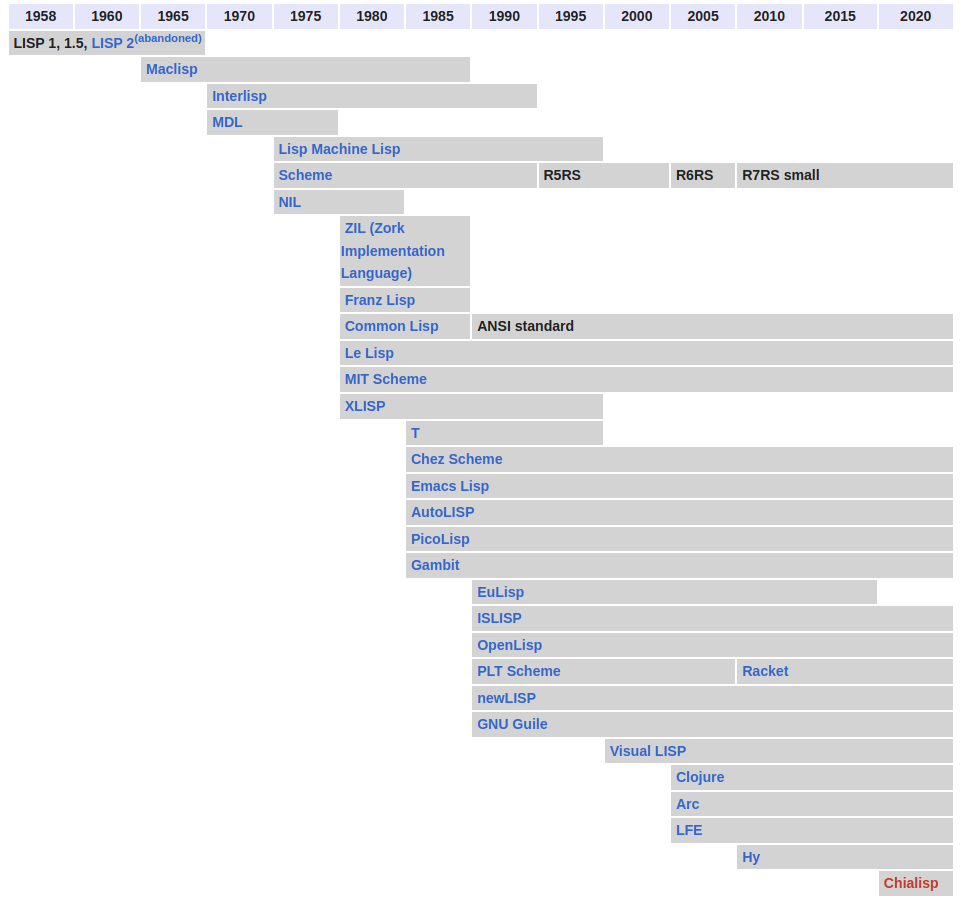
\includegraphics[width=0.7\linewidth]{bilder/lisphis.png}
            \textmd{ \tiny \url{https://en.wikipedia.org/wiki/Lisp_(programming_language)}}
	    %\caption{Enter Caption}
	    %\label{fig:enter-label}
	\end{figure}
\end{frame}

\begin{frame}
	\begin{figure}
	    \centering
	    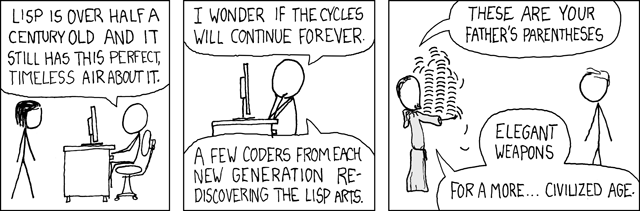
\includegraphics[width=1\linewidth]{bilder/lisp_cycles.png}
        \textmd{ \tiny \url{https://www.explainxkcd.com/wiki/index.php/297:_Lisp_Cycles}}
	    %\caption{Enter Caption}
	    %\label{fig:enter-label}
	\end{figure}
\end{frame}

\section{Features der Funktionalen Programmierung}
\begin{frame}
	\begin{itemize}
		\item Fokus auf unveränbare Daten
            \item Wenn eine Funktion pur ist, folgt: \code{Kein State -> keine Seiteneffekte}
            \item Basiert sich auf Aussagen
            \item Rerefrenzen sind Transparent:   \code{input -> output}
	\end{itemize}
\end{frame}

\begin{frame}
\frametitle{Konzepte  von FP part 1/2} 
	\begin{itemize}
		\item Höhere Geordnete Funktionen: Rufen andere Funktionen als Argumente zu übergeben oder als Ergebnisse zurückzugeben.
			\item Currying: Umwandlung von Funktionen, die mehrere Argumente annehmen, in eine Kette von Funktionen, die jeweils ein Argument akzeptieren.
			%	\item Isomorphismen: Bijektive Abbildungen zwischen Funktoren, die die Struktur vollständig bewahren und einen Informationsverlust ausschließen.
			%\item  Homomorphismen: Funktionen, die die Struktur zwischen Funktoren respektieren, aber nicht notwendigerweise bijektiv sind.
			\item Functor: \begin{itemize}
			    \item Functor: Funktion mit mehreren Argumenten in eine Kette von Funktionen umgewandelt wird, die jeweils ein Argument akzeptieren, was die teilweise Anwendung von Argumenten ermöglicht.
                    \item  Befolgt Identitätsregel und Kompositionsregel.
			\end{itemize}
	\end{itemize}
\end{frame}

\begin{frame}
\frametitle{Konzepte  von FP part 2/2} 
	\begin{itemize}
	    \item Applificat: 
	\begin{itemize}
		\item Verwendet Funktionen   '' pure\ '' oder  ''return '', um Werte in den Kontext zu bringen
		\item Nutzt den Operator \">>=\" , um Berechnungen zu verknüpfen
		\item Befolgt Identitäts- und Assoziativitätsregeln.
		\item Heißt Applikation in der Mathematik:  Anwendung einer Funktion auf ihre Argumente, wobei das Ergebnis der Funktion zurückgegeben wird. 
	\end{itemize}
	\item Monad: \begin{itemize}
		\item Abstraktion um mit Effekten wie Zustandsänderungen, Ein- und Ausgabe oder Fehlern umzugehen 
		\item ermöglicht  Berechnungen in einer sequenziellen und strukturierten Weise zu kombinieren, indem sie Werte in einem Kontext kapseln und eine einheitliche Schnittstelle für die Verarbeitung dieser Werte bereitstellen. 
		%\item Verknüpft Berechnungen in einem Kontext.
		% \item Definiert durch "return" oder "pure" und ">>=" (Bind).
		\item Befolgt Identitätsregel und Assoziativitätsregel.
	\end{itemize}
	\end{itemize}
\end{frame}

\begin{frame}
	\centering
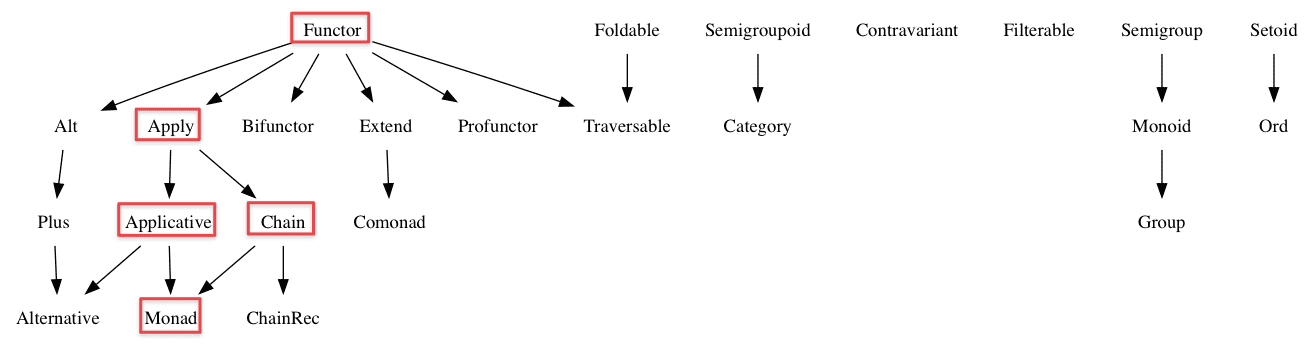
\includegraphics[scale=0.3]{bilder/monad000.png}
\textmd{\tiny \url{https://yabai.tw/category/monad/overview/}}
\end{frame}

\begin{frame}
	\centering
	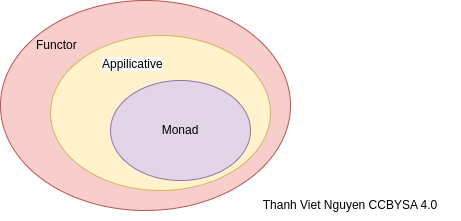
\includegraphics[scale=0.8]{bilder/functors.drawio.png}
\end{frame}

\section{Vorteile und Nachteile}
\begin{frame}
\centering
	\begin{tabular}{ |p{5cm}|p{5cm}|  }
		\hline
             \textcolor{darkgreen}{Vorteile} & \textcolor{red}{Nachteile} \\
		\hline
		Mehr Sicherheit beim Entwickeln: Nebenläufigkeit, Wartbarkeit, und Testbarkeit & in  der Regel keine Zustandskontrolle \\
            \hline 
            Paralelle Verarbeitung&  meist Speicher intensiver bei der Laufzeit  \\ 
		\hline
    Code ist in der Regel lesbarer  & Lesbarkeit $\neq$ Verständlich \\
    \hline
    Modularität & \\ 
      \hline 
            Höhere Abstraktion & \\
		\hline

 \end{tabular}
\end{frame}

\section{Anwendungsgebiete}
\begin{frame}
	\begin{itemize}
            \item Software Anwendungen 
            \item Systemkonfigurationen 
		\item Beweisasistent für Mathematische Theoreme sowie Automatische Beweisführung
		\begin{itemize}
			\item  Roqc \text{für Lisp Dialekt Liebhaber}
			\item  Lean \text{für nicht Lisp Dialekt Liebhaber}
		\end{itemize}
            \item Verarbeitung von Daten
    \end{itemize}
\end{frame}

\begin{frame}
\frametitle{Deklarative Systemkonfigurationen und Reproduzierbare Bauten}
 \begin{itemize}
		\item NixOS: GNU/Linux Distro
		\item Guix: GNU/Linux Distro, welches mit Guile Scheme Dialekt Konfiguriert wird
		\item Code als Basis für Infrastrukturen
		\item Emacs: Ein Texteditor mit vielen erweiterungen, welches mit Lisp Dialekt (Elisp)
		\item Debian GNU/Linux verwendung von OCAML für Reproduzierbare Checks
\end{itemize}

\end{frame}

\begin{frame}
    \begin{figure}
    \centering
    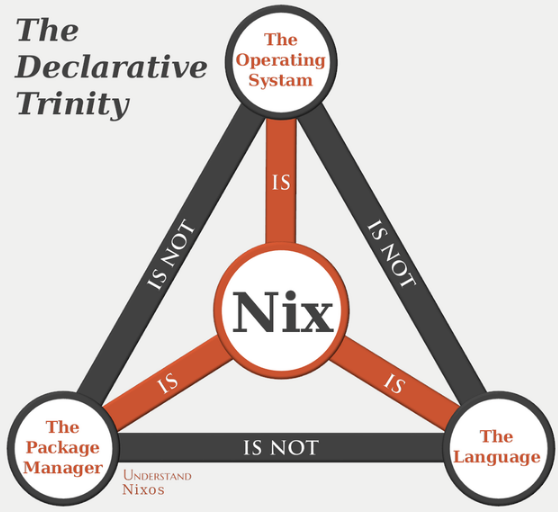
\includegraphics[width=0.7\linewidth]{bilder/nix.png}
    \textmd{\tiny \url{https://github.com/gytis-ivaskevicius/high-quality-nix-content/tree/master/memes} }
    %\caption{Caption}
    %\label{fig:enter-label}
\end{figure}

\end{frame}

\section{Fazit}
\begin{frame}
	\begin{itemize}
		\item Grundverständnis zur Funktionalen Programmiereung
		\item Lambda Kalkulus etwas kennen gelernt
		\item Einige frühere pur funktionale Programmiersprachen beinflussten moderne nicht pur funktionale Programiersprachen.
		\item Schwächen und Stärken der Funktionalen Programmierung
         \item Anwendungsgebiete die von FP geführt werden
         \item Wird in der Zukunft häufiger verwendet durch Entwickeln mit KI und Quantencomputer
         \item FP ist nicht die Lösung für alle Probleme in der Softwareentwicklung.
        \end{itemize}
\end{frame}

\begin{frame}
\centering
\frametitle{Mehr erfahren? \\ Hier sind einige Einsteiger freundliche Projekte}
\begin{itemize}
    \item Mehr über Lisp Dialekt: \url{https://docs.racket-lang.org/}
    \item Mehr über Haskell:\url{https://learnyouahaskell.github.io/}
     \item FP für weitere Programmier Sprachen: \url{https://learnfp.org/}
    \item Falls jemand nicht genug hat: \url{https://nixos.org/learn/}
    \item \code{(defun display-message () \\
  (let ((message "Falls jemand immer noch nicht genug hat: \url{https://guix.gnu.org/cookbook/}"))
(display-message)))}

\end{itemize}

\end{frame}

\begin{frame}
	\section{Quellen}
	\fontsize{8pt}{10pt}
	\centering
	\textbf{Literatur}
	\begin{itemize}
    \item Mathematics in Programming (Xinyu Liu)
\item Functional and Logic Programming (Gerhard Goos, Juris Hartmanis)
\item $\text{Revised}^6$ Report on the Algorithmic Language
Scheme (Robert Bruce Findler, Jacob Matthews)
\item Functional Programming in Java (Pierre-Yves Saumont)
\item The Design and Implemention of Programming Languages (John Hughes)
% THE DE:SIGN AND IMPLEMENTAnONOF PROGRAMMING LANGUAGES
\item A short introduction to the Lambda Calculus (Achim Jung)
\item Lambda Calculus (Tobias Nipkow) 
\item   Functional Programming with Overloading and
Higher-Order Polymorphism (Mark P. Jones)
\item A Tutorial Introduction to the Lambda Calculus (Raúl Rojas)
\item Mathematical Components (Assia Mahboubi and Enrico Tassi)
% https://ia903209.us.archive.org/12/items/working-effectively-with-legacy-code/Working.Effectively.with.Legacy.Code.pdf
 \end{itemize}
 \textbf{Weblinks}
	\begin{itemize}
		%\item \url{https://achimjungbham.github.io/pub/papers/lambda-calculus.pdf}
		\item \url{https://yabai.tw/category/monad/overview/}
        \item \url{https://bitsavers.org/pdf/mit/cadr/chinual_6thEd_Jan84/}
        \item \url{https://www.mdc-berlin.de/research/publications/pigx-reproducible-genomics-analysis-pipelines-gnu-guix}
        \item \url{https://docs.racket-lang.org/}
        \item \url{https://learnyouahaskell.github.io/}
        \item \url{https://rand.cs.uchicago.edu/cufp_2015/}
	\end{itemize}
 
\end{frame}


\end{document}
